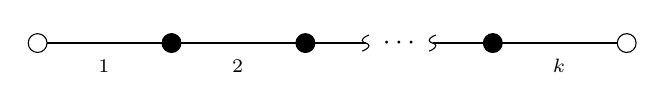
\begin{tikzpicture}[xscale=1.7,yscale=1.7]
\coordinate (a) at (0,0);
\coordinate (b) at (1,0);
\coordinate (c) at (2,0);
\coordinate (c1) at (2.45,0);
\coordinate (c2) at (2.95,0);
\coordinate (d) at (3.4,0);
\coordinate (e) at (4.4,0);
\draw (a) -- (c1);
\draw (c2) -- (e);
\node () at (2.7,0) {$\cdots$};
\node[below] () at (0.5,-0.05) {$\con_1$};
\node[below] () at (1.5,-0.05) {$\con_2$};
\node[below] () at (3.9,-0.05) {$\con_k$};
\draw plot [smooth, tension = 1] coordinates { (2.475,0.06) (2.425,0.02) (2.475,-0.02) (2.425,-0.06)};
\draw plot [smooth, tension = 1] coordinates { ({2.475+0.5},0.06) ({2.425+0.5},0.02) ({2.475+0.5},-0.02) ({2.425+0.5},-0.06)};
\draw[fill=white] (a) circle (2pt);
\draw[fill=black] (b) circle (2pt);
\draw[fill=black] (c) circle (2pt);
\draw[fill=black] (d) circle (2pt);
\draw[fill=white] (e) circle (2pt);
\end{tikzpicture}